\section{Efficiently Cleaning a Sample} \label{sampling}
%\reminder{Make sure that we do a good survey on ``sampling from a view'' and discuss them in the related work, e.g., [Frank et al., VLDB 86], [Nirkhiwale et al., VLDB 13]}
In this section, we describe how to find a relational expression $\mathcal{C}$ derived from the maintenance strategy $\mathcal{M}$ that
efficiently cleans a sample of a stale view $\widehat{S}$ to produce $\widehat{S}'$.

\subsection{Challenges}
To setup the problem, we first consider two naive solutions to this problem that will not work. 
%First, the maintenance strategy $\mathcal{M}$ can be thought of as a data cleaning procedure to clean these errors, since applying the strategy to a stale view $S$ and the delta relations $\partial \mathcal{D}$ returns an up-to-date view $S'$ without data error.
We could trivially apply $\mathcal{M}$ to the entire stale view $S$ and update it to $S'$, and then sample.
While the result is correct according to our problem formulation, it does not save us on any computation for maintenance.
We want to avoid materialization of up-to-date rows outside of the sample. 
However, the naive alternative solution is also flawed. 
For example, we could just apply $\mathcal{M}$ to the stale sample $\widehat{S}$ and a sample of the delta relations $\widehat{\partial \mathcal{D}}$. 
The challenge is that $\mathcal{M}$ does not always commute with sampling. 

\subsection{Provenance}
\label{lin}
To understand the commutativity problem, consider the maintaining a group by aggregate:
\begin{lstlisting} [mathescape,basicstyle={\scriptsize}]
SELECT videoId, count(1) FROM Log
GROUP BY videoId
\end{lstlisting}
The resulting view has one row for every distinct \texttt{videoId}.
We want to materialize a sample of $S'$, that is a sample of distinct \texttt{videoId}.
If we sample the base relation \texttt{Log} first, we do not get a sample of the view.
Instead, we get a view where every count is partial.

To achieve a sample of $S'$, we need to ensure that for each $s \in S'$ all contributing rows in subexpressions to $s$ are also sampled. 
This is a problem of row provenance \cite{DBLP:journals/vldb/CuiW03}.
Provenance, also termed lineage, has been an important tool in the analysis of materialized views \cite{DBLP:journals/vldb/CuiW03} and in approximate query processing \cite{DBLP:conf/sigmod/ZengGMZ14}.
\begin{definition}[Provenance]\label{prov}
Let $r$ be a row in relation $R$, let $R$ be derived from some other
relation $R = exp(U)$ where $exp(\cdot)$ be a relational
expression composed of the expressions defined in Section \ref{notation}.
The provenance of row $r$ with respect to $U$ is $p_U(r)$. 
This is defined as the set of rows in $U$ such that for an update to any row $u \not\in p_U(r)$, it guarantees that $r$ is unchanged.
\end{definition}

\subsection{Primary Keys}
For the relational expressions defined in the previous sections, this provenance is well defined and can be tracked using primary key rules that are enforced on
each subexpression \cite{DBLP:journals/vldb/CuiW03}. 
%Each row will have a designated primary key that will propagate to the next level of the relational tree.
We recursively define a set of primary keys for all relations in the expression tree:
\begin{definition} [Primary Key Generation]\label{pk}
For every relational expression $R$, we define the primary key attribute(s) of every expression to be:
\begin{itemize}[noitemsep]
\item Base Case: All relations (leaves) must have an attribute $p$ which is designated as a primary key. 
\item $\sigma_{\phi}(R)$: Primary key of the result is the primary key of R 
\item $\Pi_{(a_1,...,a_k)}(R)$: Primary key of the result is the primary key of R. The primary key must always be included in the projection.
\item $\bowtie_{\phi (r1,r2)}(R_1,R_2)$: Primary key of the result is the tuple of the primary keys of $R_1$ and $R_2$. 
\item $\gamma_{f,A}(R)$: The primary key of the result is the group by key $A$ (which may be a set of attributes).
\item $R_1 \cup R_2$: Primary key of the result is the union of the primary keys of $R_1$ and $R_2$
\item $R_1 \cap R_2$: Primary key of the result is the intersection of the primary keys of $R_1$ and $R_2$
\item $R_1 - R_2$: Primary key of the result is the primary key of $R_1$
\end{itemize}
For every node at the expression tree, these keys are guaranteed to uniquely identify a row.
\end{definition}
These rules define a constructive definition that can always be applied for our defined relational expressions. 

%As we will subsequently see, this primary key definition allows us to efficiently sample the relational expression.
%For the relational expressions defined in the previous section, this method will always work. 
%We only have to ensure that any projection operation $\Pi$ includes the operand's primary key, and enforcing this condition
%defines an equivalent materialized view. \reminder{Why do you emphazie the projection operation? Has this rule been defined above?}

\begin{figure}[t] \vspace{-2em}
\centering
 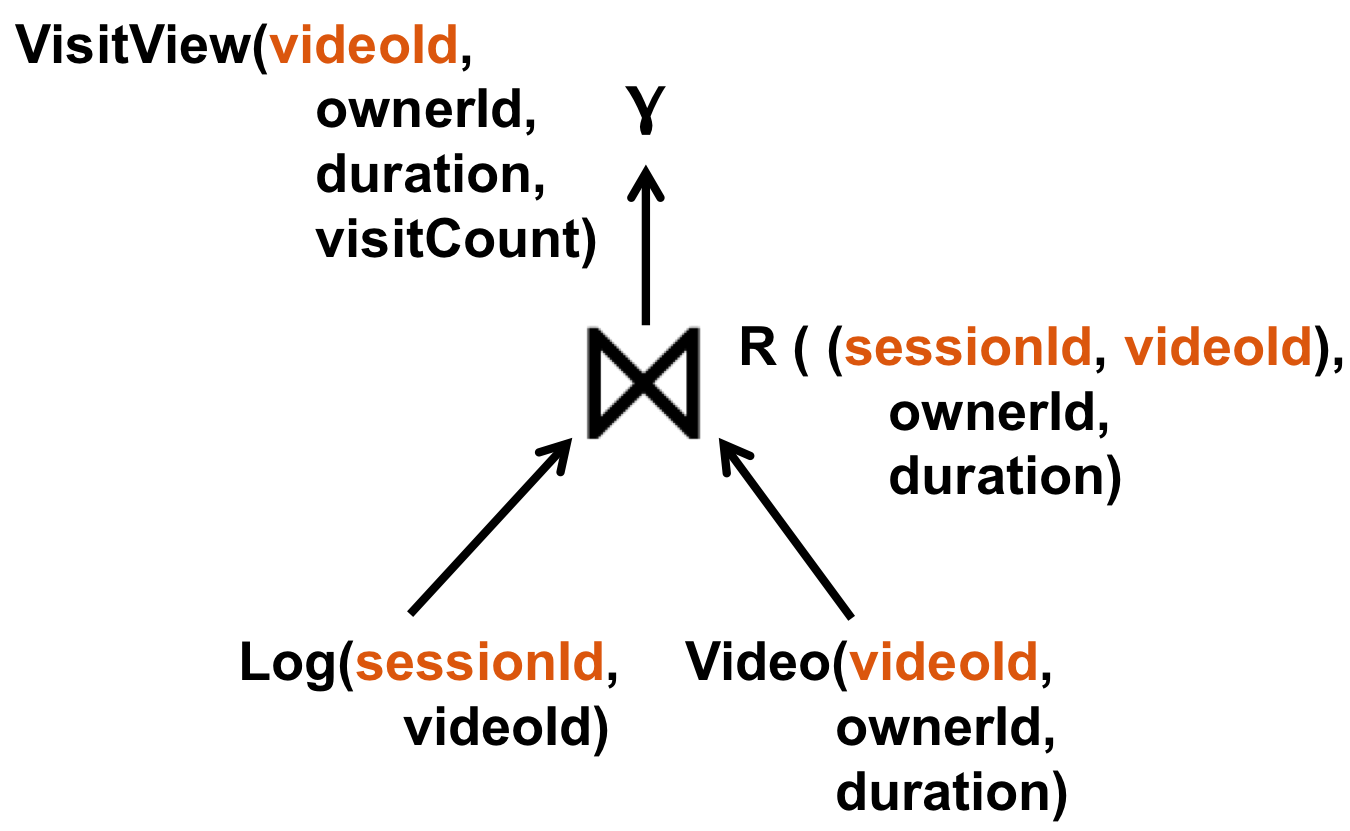
\includegraphics[scale=0.24]{figs/primary_key.png} \vspace{-.5em}
 \caption{Applying the rules described in Definition \ref{pk}, we illustrate how to assign a primary key to a view.  \label{pk-fig}}\vspace{-1.5em}
\end{figure}

\begin{example}
A variant of our running example view that does not have a primary key is:
\begin{lstlisting}[mathescape,basicstyle={\scriptsize}]
CREATE VIEW visitView AS SELECT count(1) as visitCount
FROM Log, Video WHERE Log.videoId = Video.videoId
GROUP BY videoId
\end{lstlisting}
We illustrate the key generation process in Figure \ref{pk-fig}.
Suppose there is a base relation, such as \tbl{Log}, that is missing a primary key (sessionId)\footnote{It does not make sense for Video to be missing a primary key in our running example due to the foreign key relationship}.
We can add this attribute by generating an increasing sequence of integers for each record in \tbl{Log}. 
Since both base tables \tbl{Video} and \tbl{Log} have primary keys videoId and sessionId respectively,
the result of the join will have a primary key (videoId, sessionId).
Since the group by attribute is videoId, that becomes the primary key of the view.
\end{example}

\subsection{Hashing Operator}
\label{push}
The primary keys allow us to determine the set of rows that contribute to a row $r$ in a derived relation.
If we have a deterministic way of mapping a primary key to a Boolean, we can ensure that all contributing rows are also sampled. 
To achieve this we use a hashing procedure.
Let us denote the hashing operator $\eta_{a, m}(R)$. 
For all tuples in R, this operator applies a hash function whose range is $[0,1]$ to primary key $a$ (which may be a set) and selects those records with hash less than or equal to $m$.
If the hash function is sufficiently uniform, then the condition $h(a) \le m$ is true for a fraction of approximately $m$ of the rows. 
%This definition is without loss of generality for uniform hash function, as if we have a hash function whose range is the set of integers (as implemented in MySQL or Apache Hive) we can take the absolute value and divide by the maximum integer mapping this range back $[0,1]$. 

To avoid materializing extra rows, we push down the hashing operator through the expression tree.
The further that we can push $\eta$ down, the more operators (i.e., above the sampling) can benefit.
This push down is analogous to predicate push-down operations used in query optimizers. 
In particular, we are interested in finding an optimized relational expression that materializes an identical sample before and after the push down.

We formalize the push down rules below:
\begin{definition}[Hash push down]
For a derived relation $R$, the following rules can be applied to push $\eta_{a, m}(R)$ down the expression tree. 
\begin{itemize}[noitemsep]
\item $\sigma_{\phi}(R)$: Push $\eta$ through the expression.  
\item $\Pi_{(a_1,...,a_k)}(R)$: Push $\eta $ through if $a$ is in the projection.
\item $\bowtie_{\phi (r1,r2)}(R_1,R_2)$: No push down in general. There are special cases below where push down is possible.
\item $\gamma_{f,A}(R)$: Push $\eta $ through if $a$ is in the group by clause $A$.
\item $R_1 \cup R_2$: Push $\eta $ through to both $R_1$ and $R_2$
\item $R_1 \cap R_2$: Push $\eta $ through to both $R_1$ and $R_2$
\item $R_1 - R_2$: Push $\eta $ through to both $R_1$ and $R_2$
\end{itemize}
\end{definition}
In special cases, we can push the hashing operator down through joins. 
Given the hash function $\eta_{a, m}(R)$:
\vspace{.25em}

{\noindent \textbf{Equality Join:}} If the join is an equality join and $a$ is one of the attributes in the equality join condition $R_1.a = R_2.b$, then $\eta$ can be pushed down to both $R_1$ and $R_2$. On $R_1$ the pushed down operator is $\eta_{a, m}(R_1)$ and on $R_2$ the operator is $\eta_{b, m}(R_2)$. 

\vspace{.25em}

{\noindent \textbf{Foreign Key Join:}} If we have a join with two foreign-key relations $R_1$ (fact table with foreign key $a$) and $R_2$ (dimension table with primary key $b \subseteq a$) and we are sampling the key $a$, then we can push the sampling down to $R_1$. This is because we are guaranteed that for every $r_1\in R_1$ there is only one $r_2 \in R_2$. 

\vspace{0.25em}

\begin{theorem}
Given a derived relation $R$, primary key $a$, and the sample $\eta_{a, m}(R)$.
Let $S$ be the sample created by applying $\eta_{a, m}$ without push down and 
$S'$ be the sample created by applying the push down rules to $\eta_{a, m}(R)$.
$S$ and $S'$ are identical samples with sampling ratio $m$.
\end{theorem}
\begin{proof}[Sketch]
We can prove this by induction.
The base case is where the expression tree is only one node, trivialy making this true.
Then, we can induct considering one level of operators in the tree.
$\sigma, \cup, \cap, -$ clearly commute with hashing the key $a$ allowing for push down.
$\Pi$ commutes only if $a$ is in the projection.
For $\bowtie$, a sampling operator on $Q$ can be pushed down if $a$ is in either $k_r$ or $k_s$, or if there is a constraint that links $k_r$ to $k_s$ (a foreign key constraint).
For group by aggregates, if $a$ is in the group clause (i.e., it is in the aggregate) then a hash of the operand filters all rows that have $a$ which is sufficent to materialize the derived row.
\end{proof}

{\noindent \textbf{Limitations: }} There are two basic cases where push down fails: joins and group by aggregates. 
Consider the all-pairs join $R \times S$, a single hash of the keys $(k_s, k_r)$ cannot be pushed down to either A or B. 
If we pushed down the operator, we would get a join of a sample of $R$ and a sample of $S$ which would not be the sample as a sample of $R \times S$.
For group by aggregates, if the hashing attribute is not in the group clause (i.e., it is in the aggregate) then push down will not work since the provenance is not uniquely determined.

\subsection{Efficient View Cleaning}
If we apply the hashing operator to $\mathcal{M}$, we can get an optimized cleaning expression $\mathcal{C}$ that avoid materializing unnecessary rows. 
When applied to a stale sample of a view $\widehat{S}$, the database $\mathcal{D}$, and the delta relations $\partial \mathcal{D}$, it produces an up-to-date sample with sampling ratio $m$:
\[
\widehat{S}' = \mathcal{C}(\widehat{S},\mathcal{D},\partial \mathcal{D})
\]
Thus, it addresses Problem 1 from the previous section.

\begin{figure}[t] \vspace{-2em}
\centering
 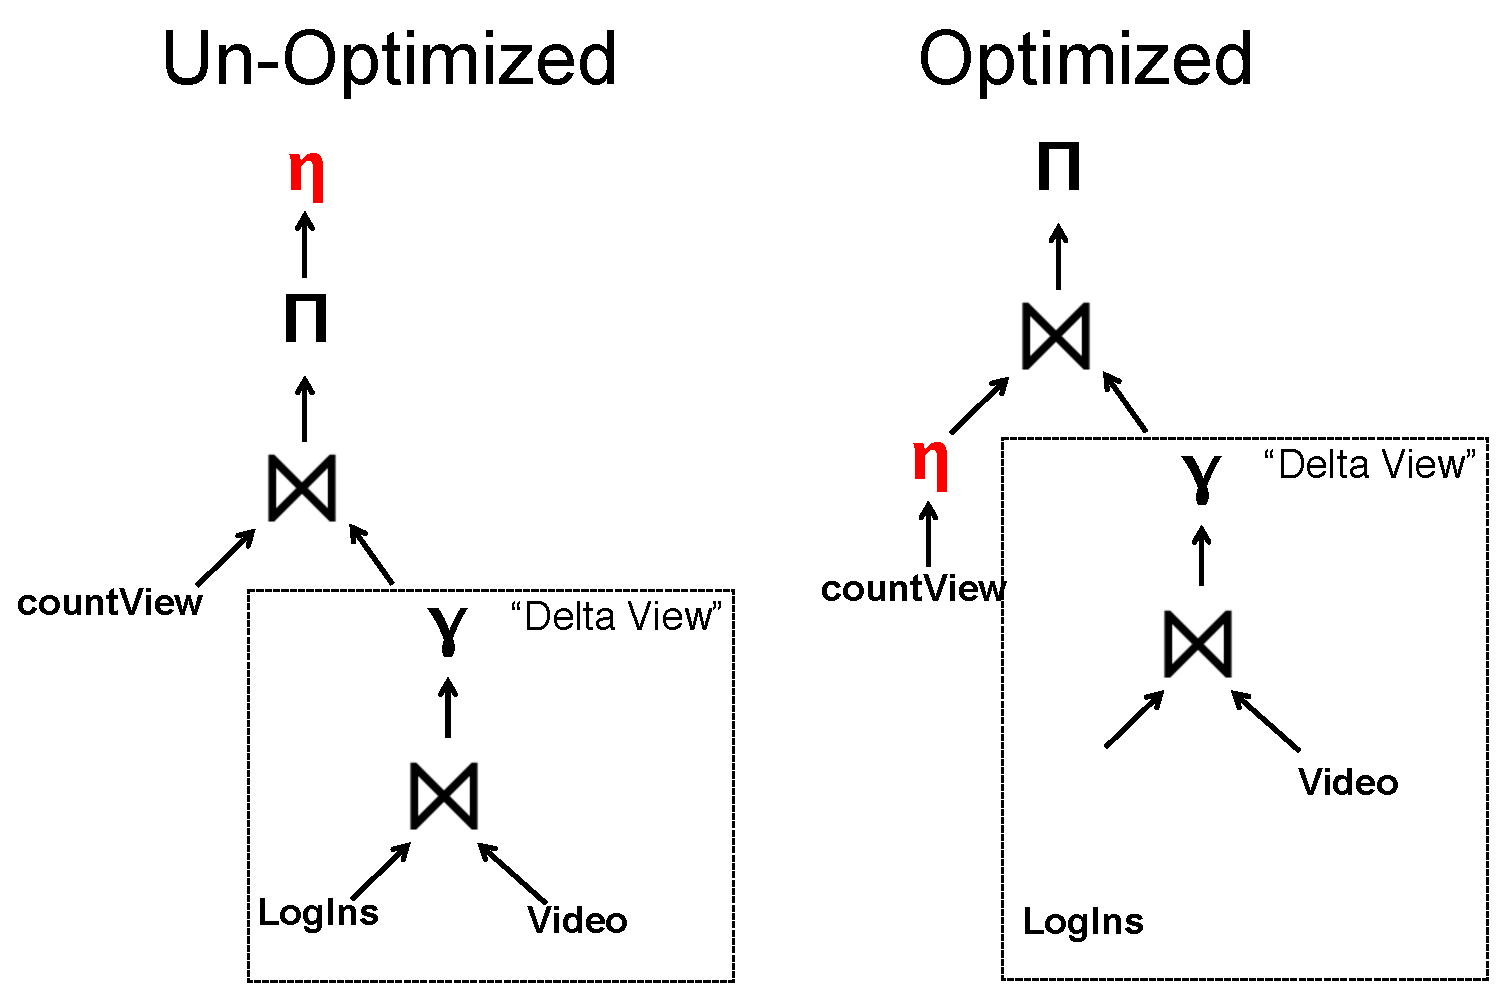
\includegraphics[scale=0.22]{figs/example_expression_tree_2.pdf} \vspace{-.5em}
 \caption{Applying the rules described in Section \ref{push}, we illustrate how to optimize the sampling of our example maintenance strategy. \label{exexpr2}}\vspace{-1em}
\end{figure}

\begin{example}
We illustrate our proposed approach on our example view \texttt{visitView} (Figure \ref{exexpr2}). 
The primary key for the view is the tuple (\texttt{videoId}) making that the primary key of the MV.
We start by applying the hashing operator to this key.
The next operator we see in the expression tree is a projection that increments the \texttt{visitCount} in the view, and this allows
for push down since primary key is in the projection.
The second expression is a hash of the equality join key which merges the aggregate from the ``delta view'' to the old view allowing us to push down on both branches of the tree using our special case for equality joins.
On the left side, we reach the stale view so we stop.
On the right side, we reach the aggregate query (count) and since the primary key is in group by clause, we can push down the sampling.
Then, we reach another point where we hash the equality join key allowing us to push down the sampling to the relations \tbl{LogIns} and \tbl{Video}.
\end{example}

\subsection{Corresponding Samples}
We started with a uniform random sample $\widehat{S}$ of the stale view $S$.
The hash push down allows us to efficiently materialize the sample $\widehat{S}'$.
$\widehat{S}'$ is a uniform random sample of the up-to-date view S.
While both of these samples are uniform random samples of their respective relations, 
the two samples are correlated since $\widehat{S}'$ is generated by cleaning $\widehat{S}$.
In particular, our hashing technique ensures that the primary keys in $\widehat{S}'$ depend on the primary keys in $\widehat{S}$.
Statistically, this positively correlates the query result $q(\widehat{S}')$ and $q(\widehat{S})$. 
We will see how this property can be leveraged to improve query estimation accuracy (Section \ref{re}). 

\begin{property}[Correspondence]
Suppose $\widehat{S'}$ and $\widehat{S}$ are uniform samples of $S'$ and $S$, respectively.  Let $u$ denote the primary key. We say $\widehat{S'}$ and $\widehat{S}$ correspond if and only if:
\vspace{-.25em}
\begin{itemize}[noitemsep]
\item Uniformity: $\widehat{S'}$ and $\widehat{S}$ are uniform random samples of $S'$ and $S$ respectively with a sampling ratio of $m$
\item Removal of Superfluous Rows: $D = \{\forall s \in \widehat{S} \nexists s' \in S': s(u) = s'(u)\}$, $D \cap \widehat{S'} = \emptyset$ 
\item Sampling of Missing Rows: $I = \{\forall s' \in \widehat{S'} \nexists s \in S: s(u) = s'(u)\}$, $\mathbb{E}(\mid I \cap \widehat{S'} \mid) = m\mid I \mid $ 
\item Key Preservation for Updated Rows: For all $s\in \widehat{S}$ and not in $D$ or $I$, $s' \in \widehat{S}': s'(u) = s(u)$.
\end{itemize}
\vspace{-.25em}
\label{correspondence}
\end{property}






